\chapter{Background}
\label{cha:background}

The purpose of this chapter is to provide a comprehensive description of the
attacks that we aim to mitigate with the implemented security features. We start
by listing the main threats and discussing how they can disrupt the execution flow
of the system to cause damage. Secondly, we describe possible solutions to these
types of threats focusing on Control Flow Integrity, its purpose, and how this security
measure can effectively detect and prevent control flow hijacking attacks.
Lastly, we present related works discussing the differences between them and the
novel solution proposed in this thesis.

\section{Control Flow Hijacking Attacks}
\label{sec:background_cfa}

Control flow hijacking attacks are a category of cyber attacks that aim at
disrupting the normal execution flow of a program. Normally, some code follows
one or more paths during execution, control flow attacks aim at modifying such flow
by transferring control to existing or injected malicious code. The purpose of
these types of attacks is to alter the program's flow to leak information, gain higher
privileges, execute arbitrary code, or, in general, hijack the system.

This project is focused primarily on detecting and preventing control flow hijacking
attacks on \textit{RISC-V}-based embedded systems. Here, we provide a list of
these types of threats showcasing how they can affect the execution path to
impact the system.

\subsection{Code Reuse Attacks}
\label{subsec:background_codereuse}

\textit{Code Reuse Attacks} are a class of exploit techniques in which an
attacker uses existing, legitimate code within a program to execute malicious actions,
circumventing protections like non-executable memory regions. These attacks exploit
the fact that many software protections assume that code residing in executable regions
of memory is safe, and they focus instead on preventing the execution of data in
memory. By leveraging already present and authorized code snippets, attackers
avoid introducing new code, making detection and prevention more challenging.

\begin{wrapfigure}
  [23]{r}{.35\textwidth}
  \centering
  \def\stackalignment{r}\stackunder{ 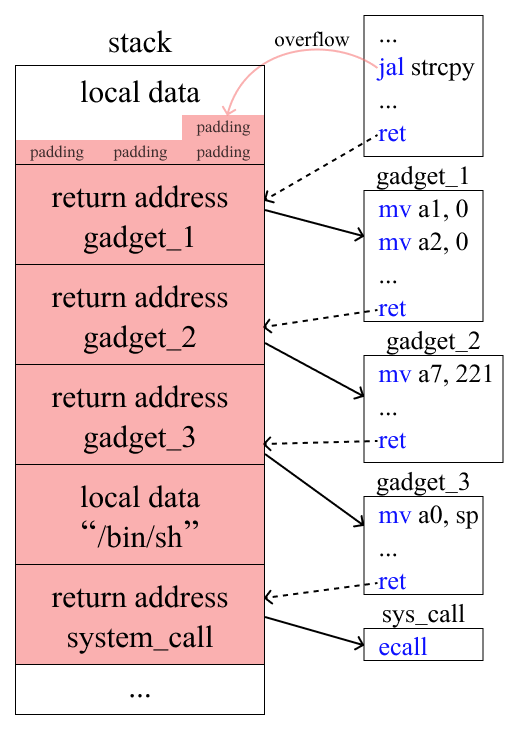
\includegraphics[width=\linewidth]{images/rop.png} } %
  {\scriptsize \parbox[t]{\linewidth}{Source: \href{http://dx.doi.org/10.1145/3320269.3384738}{Return-Oriented Programming on RISC-V}\cite{rop}}}
  \caption{\textit{Return-Oriented Programming} principle}
  \label{fig:rop}
\end{wrapfigure}

One common example of a \textit{Code Reuse Attack} is \textit{Return-Oriented
Programming} (ROP). In ROP, an attacker utilizes a sequence of ``gadgets'', which
are small chunks of code ending in a return instruction. These gadgets are
typically harvested from the binary or shared libraries of the targeted program
and perform specific operations. By chaining gadgets together through careful manipulation
of the program's stack, the attacker creates a sequence of instructions that
accomplish a broader malicious goal, such as disabling security mechanisms,
executing shellcode, or gaining unauthorized access. Figure \ref{fig:rop}
depicts the principle of \textit{Return-Oriented Programming}.

\textit{Jump-Oriented Programming} (JOP) is a variation of ROP, where instead of
relying on return instructions, attackers rely on jump or call instructions to
chain gadgets. Similarly to ROP, these approaches exploit the control flow of
the application without introducing new code into the memory space.

\textit{Code Reuse Attacks} are particularly dangerous because they bypass certain
forms of security, such as signature-based detection mechanisms and runtime
protections that rely on identifying or blocking the introduction of foreign
code. Techniques like Address Space Layout Randomization attempt to mitigate these
attacks by randomizing the locations of code in memory, but attackers may
combine information leakage vulnerabilities or brute force techniques to bypass
Address Space Layout Randomization and successfully locate the needed gadgets.

The sophistication of \textit{Code Reuse Attacks} lies in their ability to manipulate
a program's legitimate functionality to achieve unintended behavior while leveraging
the program's permissions and resources. This makes them a preferred method for
attackers seeking reliability in their exploits.

\subsection{Stack Smashing Attacks}
\label{subsec:background_stacksmashing}

A \textit{Stack Smashing Attack} is a type of exploit that targets
vulnerabilities in a program's use of memory, specifically the stack, to gain
unauthorized access or control over the program's execution. It typically occurs
in applications that improperly handle input data, allowing attackers to
overwrite parts of the stack with their own crafted data.

The attack begins with exploiting a buffer overflow vulnerability, which arises when
a program allocates a fixed-size buffer on the stack to store user input but fails
to check whether the input exceeds the buffer's size. When the attacker provides
input that surpasses this limit, the excess data spills over into adjacent memory
regions of the stack. These regions might contain critical information, such as the
function's saved return address or local variables.

By carefully crafting the overflowing input, an attacker can overwrite the saved
return address with the address of malicious code previously injected into the
memory or a code reuse sequence. When the function attempts to return, it jumps
to the attacker-controlled location instead of the intended one. This redirection
allows the attacker to execute arbitrary instructions, potentially leading to
unauthorized access, data leakage, or system compromise.

\textit{Stack Smashing Attacks} are particularly devastating because they exploit
the very structure of program execution. They are often used to bypass security
measures and gain control of systems, especially in older or poorly secured software.

\subsection{Function Pointer Overwrite Attacks}
\label{subsec:background_pointeroverwrite}

\textit{Function Pointer Overwrite Attacks} exploit vulnerabilities in programs where
an attacker can modify memory regions containing function pointers to redirect the
control flow of the application to malicious code. Function pointers are
variables that store the address of a function and are used in programming
languages like \textit{C} and \textit{C++} to enable dynamic function calls. If these
pointers are improperly managed or located in memory regions susceptible to manipulation,
such as the stack, they become targets for attackers.

The attack begins by identifying a vulnerability that allows writing arbitrary data
to memory, such as a buffer overflow, use-after-free condition, or format string
vulnerability. Once access to the function pointer's memory location is obtained,
the attacker overwrites it with the address of their chosen code. This address could
point to injected shellcode, a sequence of gadgets crafted to perform unintended
actions, or malicious functions in shared libraries.

When the program later attempts to use the overwritten function pointer to make a
call, control flow is redirected to the attacker-specified address instead of
the intended function. This allows the attacker to execute arbitrary code or alter
the behavior of the application to perform tasks such as privilege escalation,
information leakage, or system compromise.

Function pointer overwrites are particularly dangerous because they exploit the flexibility
and power of dynamic function calls, which are common in modular and object-oriented
programming. Attackers often pair this technique with other vulnerabilities,
such as memory corruption, to achieve a reliable exploit.

\subsection{Virtual Table Hijacking Attacks}
\label{subsec:background_virtualtable}

\textit{Virtual Table (vtable) Hijacking Attacks} exploit vulnerabilities in programs
that use polymorphism in object-oriented programming, particularly in languages
like \textit{C++} that implement virtual functions. These attacks target the
virtual table which is a structure that supports dynamic method calls in
polymorphic objects. The \textit{vtable} is essentially an array of function
pointers associated with a class, pointing to the implementations of the class'
virtual functions. Each polymorphic object contains a pointer, often called a
\textit{vtable} pointer or \textit{vptr}, that references the class' \textit{vtable}.
When a virtual function is called on the object, the function pointer in the \textit{vtable}
is dereferenced to invoke the corresponding method.

In a \textit{Virtual Table Hijacking Attack}, the attacker exploits memory
vulnerabilities, such as a buffer overflow or use-after-free to gain unauthorized
write access to the \textit{vptr} or the \textit{vtable} itself.

Once the attacker has control, they overwrite the \textit{vptr} of an object with
a pointer to their malicious \textit{vtable} or modify function pointers in the
legitimate \textit{vtable} to point to attacker-controlled code. When the
program invokes a virtual function on the compromised object, it executes the attacker's
code instead of the intended method. This redirection allows the attacker to
perform arbitrary actions, such as executing injected shellcode, bypassing
security checks, or escalating privileges.

\textit{Virtual Table Hijacking Attacks} are especially dangerous because they
exploit a core mechanism of object-oriented programming, making them difficult to
detect. Additionally, they can bypass certain security measures, as the attack
typically occurs within legitimate program memory and uses expected program
structures like \textit{vtables} and \textit{vptrs}.

\subsection{Dynamic Linking Attacks}
\label{subsec:background_dynamiclinking}

\textit{Dynamic Linking Attacks} exploit the mechanism by which programs resolve
and use shared libraries at runtime. Many modern systems use dynamic linking to reduce
memory usage and facilitate updates by allowing multiple programs to share the same
libraries rather than including them in their executables. During execution, the
operating system's dynamic linker resolves symbols in the program's code to corresponding
functions or variables in the shared libraries. This process, while efficient,
introduces a potential attack vector when not properly secured.

An attacker leveraging a \textit{Dynamic Linking Attack} typically manipulates how
or where the dynamic linker resolves these dependencies. One common method is to
exploit weaknesses in the search order of libraries. If a program relies on a library
without specifying its exact path or uses a default path search mechanism, an
attacker can introduce a malicious library in a location searched earlier, replacing
the legitimate one. This library might mimic the interface of the expected
library while performing malicious activities, such as executing shellcode or stealing
sensitive data.

Another approach involves manipulating environment variables like \textit{LD\_PRELOAD}.
Such a variable forces the dynamic linker to load specific libraries before others,
overriding the default linking process. An attacker who gains control of these variables
can inject a malicious library that intercepts or replaces critical function calls.

\textit{Dynamic Linking Attacks} are particularly dangerous because they often
blend with legitimate program behavior, making detection challenging. They can
be used to escalate privileges, steal information, or execute arbitrary code
within the context of the targeted application.

\subsection{Indirect Branch Attacks}
\label{subsec:background_indirectbranch}

\textit{Indirect Branch Attacks} exploit the control flow of a program by
targeting indirect branch instructions, which are used to transfer execution to an
address determined at runtime. Indirect branches are commonly found in
constructs like function pointers, virtual table lookups, and dynamic jump
tables. Unlike direct branches, where the target address is fixed at compile-time,
indirect branches are flexible and rely on runtime-determined values stored in registers
or memory. This flexibility makes them a target for attackers seeking to
redirect program execution.

These attacks typically involve corrupting the data used to calculate the target
of the indirect branch. For example, in an indirect function call via a function
pointer, an attacker might use a memory corruption vulnerability such as a buffer
overflow to overwrite the function pointer with an address of their choosing.

Attackers can also exploit jump tables used to implement features like switch statements.
By corrupting the memory that stores jump table entries, they can redirect execution
to arbitrary addresses when the program uses the table to determine the branch target.

\textit{Indirect Branch Attacks} are particularly dangerous because they can
bypass many conventional control flow defenses. They often do not introduce new code
into memory, instead relying on existing executable code, which allows them to evade
protections like Data Execution Prevention. Additionally, they leverage the program's
legitimate branching mechanisms, making them harder to detect and mitigate.

\section{Control Flow Hijacking Attack Mitigations}
\label{sec:background_mitigation}

Given the impact that control flow hijacking attacks may have on a program's execution
the necessity for security measures increased drastically over the last years.
Many techniques have been devised to address this specific kind of attack. In this
section, we describe the security measures currently used to prevent these
threats giving great importance to Control Flow Integrity which is the security
feature implemented within this project.

\subsection{Address Space Layout Randomization (ASLR)}
\label{subsec:background_aslr}

\textit{Address Space Layout Randomization} (ASLR) is a security technique used
to protect systems against memory corruption attacks by randomizing the memory
locations of key data areas within a process. These areas include the stack,
heap, dynamic libraries, and executable code. By introducing unpredictability into
the memory layout, ASLR significantly complicates the exploitation of
vulnerabilities that rely on knowing or predicting the addresses of specific
code or data structures.

ASLR operates by changing the base addresses of these memory regions each time a
program is executed. For example, the starting address of the stack might be
shifted by a random offset on every program launch, making it nearly impossible for
an attacker to predict where specific variables or return addresses are stored.
Similarly, the heap and dynamically loaded libraries are relocated to different positions
in memory, disrupting any attempt to exploit predictable layouts.

This technique is particularly effective against attacks such as buffer
overflows, \textit{Return-Oriented Programming}, and \textit{Jump-Oriented
Programming}. Without knowing the exact location of data or executable code,
attackers face significant difficulty in crafting reliable exploits. They need to
resort to brute-force attacks, repeatedly guessing memory addresses, or leverage
memory-leak vulnerabilities that may be present in the program.

However, note that on systems with insufficient randomness, the predictability of
memory layouts may still be exploited. Despite this, \textit{Address Space
Layout Randomization} remains a valid security practice.

\subsection{Data Execution Prevention (DEP)}
\label{subsec:background_dep}

\textit{Data Execution Prevention} (DEP) is a security feature designed to
prevent code from being executed in regions of memory that are intended to store
data. Its primary purpose is to mitigate the risk of exploits that rely on executing
malicious code injected into non-executable regions, such as buffer overflow
attacks, where attackers attempt to inject and run arbitrary code within areas like
the stack or heap.

Normally, data sections of memory are writable but not executable, while code sections
are executable but not writable. This separation ensures that code is only
executed in areas where it is supposed to run, like the code segment, while
other areas are reserved for data storage.

DEP works by marking certain memory regions as non-executable, meaning that even
if an attacker successfully injects code into these regions, the system will
prevent it from executing. For instance, in the case of a buffer overflow, if an
attacker tries to overwrite the return address with a pointer to malicious code stored
in the stack, DEP will prevent the execution of that code, as the stack is designated
as non-executable. On the other hand, for an attacker is impossible to inject code
in an executable memory region as such region would be non-writable.

While DEP provides a significant layer of protection against certain exploits,
it is not a complete solution. For example, attackers may still bypass DEP
through techniques like \textit{Return-Oriented Programming}. Despite this, \textit{Data
Execution Prevention} remains a valid defense mechanism, as it helps to prevent a
wide range of exploits.

\subsection{Stack Canary}
\label{subsec:background_canaries}

The \textit{Stack Canary} is a security mechanism designed to protect against stack-based
buffer overflow attacks. The concept of a \textit{Stack Canary} is based on placing
a special value, known as the ``canary'', between the local variables of a function
and its return address on the stack. This canary value acts as a sentinel, designed
to detect any buffer overflow that overwrites it.

Typically the canary value is placed right before the return address during a function
call. When a function returns, the program checks whether the canary value has been
altered. If an attacker attempts to exploit a buffer overflow and overwrite the
return address, they will likely change the canary value as well. When the
function attempts to return, the altered canary is detected, and the program
takes a protective action such as terminating the process. This prevents the attacker
from successfully hijacking the control flow. Figure \ref{fig:canary} provides a
visual representation of the positioning of the \textit{Stack Canary} inside the
stack.

The canary is chosen randomly during program startup and is kept secret, making
it difficult for attackers to predict and overwrite. This randomness adds a layer
of protection by ensuring that an attacker cannot easily craft an exploit to target
the canary directly.

\begin{wrapfigure}
  [19]{r}{.25\textwidth}
  \centering
  \def\stackalignment{r}\stackunder{ 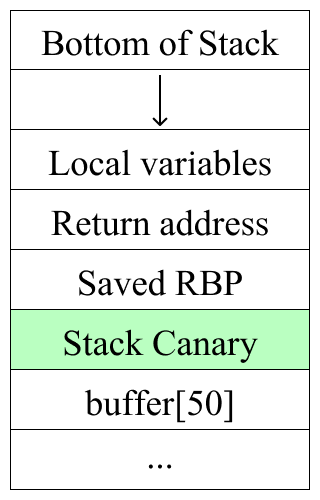
\includegraphics[width=\linewidth]{images/canary.png} } %
  {\scriptsize \parbox[t]{\linewidth}{}}
  \caption{\textit{Stack Canary} positioning}
  \label{fig:canary}
\end{wrapfigure}

While \textit{Stack Canaries} provide a strong defense against many buffer overflow
attacks, they are not foolproof. Attackers may attempt to bypass canaries by exploiting
vulnerabilities that do not trigger a canary check, such as in cases of non-stack
buffer overflows or when the attacker has partial control over the canary value
itself. However, \textit{Stack Canaries} significantly increase the difficulty of
exploiting stack-based buffer overflows and are a valuable tool in defending against
this class of vulnerabilities.

\subsection{Control Flow Integrity (CFI)}
\label{subsec:background_cfi}

\textit{Control Flow Integrity} (CFI) is a security mechanism designed to prevent
attackers from hijacking the control flow of a program. Its primary goal is to
ensure that a program executes along its intended paths and that any attempt to
divert execution to arbitrary, malicious code is detected and blocked. CFI
achieves this by enforcing constraints on the control flow of a program, specifically
the transfer of control during function calls and returns.

During the compilation process, CFI validates all possible paths a program can
take during execution. This contains the legitimate destinations for all indirect
control transfers, such as function pointers or virtual function calls, and the valid
locations for return instructions. A commonly used technique to do so is
extracting the Control Flow Graph (CFG) of the executable which is a graph that
depicts all possible paths the program can take. Figure \ref{fig:cfg} represents
an example of the extraction of a Control Flow Graph. By comparing the actual
execution flow against the predefined valid paths, CFI can detect when a program
deviates from its expected behavior and take countermeasures.

At runtime, \textit{Control Flow Integrity} enforces two main types of protection:
\begin{itemize}
  \item Forward Edge Protection: This protects against attacks that attempt to
    divert execution to unintended code via indirect function calls or jumps as
    in the example of \textit{Jump-Oriented Programming}. When a program
    attempts to execute an indirect control flow instruction, CFI checks whether
    the target of the instruction is a valid destination or not to determine the
    validity of the instruction. This control is further explained in section
    \ref{subsubsec:background_forward};

  \item Backward Edge Protection: This ensures that return instructions execute
    at the correct locations. \textit{Return-Oriented Programming} attacks, for example,
    hijack return addresses to redirect control flow to malicious code. CFI prevents
    such attacks by validating that a return address corresponds to an allowed function
    return point, ensuring that execution returns to a legitimate location. This
    control is further explained in section \ref{subsubsec:background_backward}.
\end{itemize}

To enforce \textit{Control Flow Integrity}, the program is instrumented with additional
runtime checks that validate each control transfer. These checks should be
lightweight and efficient as they need to reduce the performance overhead due to
the extra verification steps as much as possible.

CFI is highly effective against several attacks, including buffer overflow exploits,
\textit{Return-Oriented Programming}, and \textit{Jump-Oriented Programming},
all of which rely on manipulating control flow to execute arbitrary instructions.
By blocking any control flow that does not align with the intended program execution,
CFI makes it much harder for attackers to execute these attacks successfully.

Despite its effectiveness, CFI is not foolproof. Attackers can sometimes bypass
CFI protections if they can manipulate the Control Flow Graph, exploit information
leaks, or find ways to corrupt the runtime checks. However, CFI provides a
powerful defense by ensuring that a program's control flow adheres strictly to
predefined, legitimate paths, greatly reducing the success of many advanced
exploits.

Overall, \textit{Control Flow Integrity} is an essential part of modern security
practices, offering a robust way to protect programs from control flow hijacking
and ensuring that software behaves as intended even in the presence of sophisticated
attacks.

\begin{figure}
  \centering
  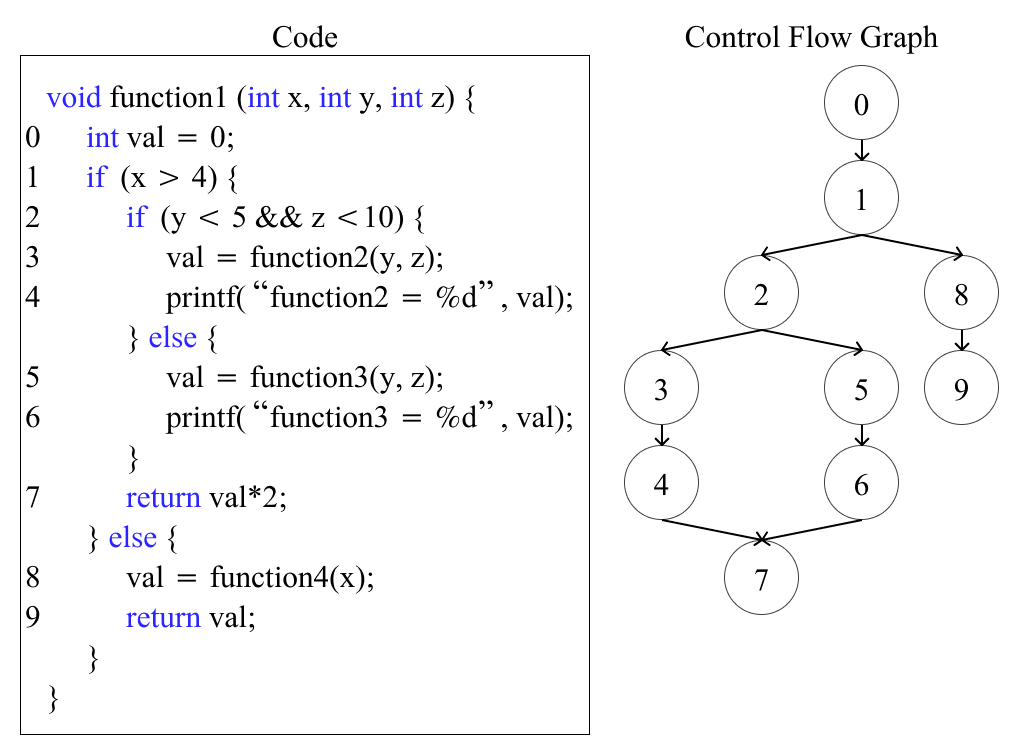
\includegraphics[width=.6\linewidth]{images/cfg.png}
  \caption{Control Flow Graph extraction}
  \label{fig:cfg}
\end{figure}

\subsubsection{Forward Edge Protection}
\label{subsubsec:background_forward}

\textit{Forward Edge Protection} is the part of Control Flow Integrity that
determines the validity of jump and call transfer instructions. This protection is
crucial to detect and prevent attacks such as \textit{Jump-Oriented Programming}.

The first part of this process involves identifying all the forward edges that
need protection. This can be done by inspecting the source code either manually or
with tools. Once the edges have been identified we must construct a Control Flow
Graph which lists all the valid transfer of control within the executable. Such a
graph is needed to inspect runtime control transfer instructions and determine if
they stay within the boundaries of the expected execution path of the program.
Direct jump instructions are defined at compile time so, to determine the source
and destination of each instruction, we can simply look at a dump of the binary.
On the other hand, the targets of indirect jump instructions are calculated at
runtime so we need further inspection to determine all the possible targets. To achieve
this result we can perform an execution simulation to gather information about the
source and destination of each indirect jump instruction.

Moreover, we need to instrument the code by adding instructions that allow the
Control Flow Integrity enforcer to examine each control transfer during
execution. At runtime, whenever the code tries to perform a jump instruction, the
source and destination of such instruction are checked. If the inspected pair is
legal according to the Control Flow Graph the instruction is allowed and the
execution continues normally. On the other hand, if the pair is not part of the
CFG, we need to halt the program to prevent the execution of malicious code.

It is easy to see how \textit{Forward Edge Protection} prevents threats such as
\textit{Jump-Oriented Programming}. If an attacker tries to tamper with the
target of a control transfer instruction to execute a gadget or some malicious
code that was previously injected we can be sure that such targets are not part
of the Control Flow Graph, thus the attack will be detected and prevented.

Note that there are other ways to implement \textit{Forward Edge Protection}. An
example is using \textit{Landing Pads} which are specific blocks of code
designed to handle a control flow transfer safely and predictably. The idea is to
use a \textit{Landing Pad} to check that the target of the jump is a valid
function or routine within the legitimate Control Flow Graph instead of directly
jumping to arbitrary locations. If the target is invalid, the \textit{Landing
Pad} can trigger a security response, such as halting execution or triggering an
alert.

\textit{Landing Pads} can be implemented with minimal runtime performance overhead
and allow for flexible control over indirect control flow while maintaining security.
However, they are typically more context-specific and not as widely applicable as
other techniques such as Control Flow Graph validation.

\subsubsection{Backward Edge Protection}
\label{subsubsec:background_backward}

\textit{Backward Edge Protection} is the part of Control Flow Integrity that determines
the validity of return instructions. This protection is crucial to detect and
prevent attacks such as \textit{Return-Oriented Programming}.

Unlike Forward Edge Protection we do not need to predefine valid targets at compile
time. This is because, during execution, the code will eventually perform a jump
instruction and, as a consequence, it will eventually return to the same
function that previously made the jump. This part of Control Flow Integrity focuses
on guaranteeing that every function returns to its expected caller.

\textit{Backward Edge Protection} is usually enforced with a shadow stack which
is a separate stack used to store return addresses. The idea is that every time that
a jump instruction is performed we insert the corresponding return address inside
the shadow stack. By doing this, we can effectively compare the last return address
inserted in the stack with the address to which a return instruction is trying to
transfer control. If the addresses match we know that the return address is
correct and thus the instruction is safe and can be performed. On the other hand,
if the addresses mismatch, we terminate the program to prevent the execution of malicious
code.

Say that an attacker performs a buffer overflow attack to overwrite the return address
stored in the stack so that it points to some malicious code or a gadget. As
soon as the current function tries to perform the return instruction we see that
the return address and the address stored in the shadow stack are not the same. This
happens because the current function was called neither by the malicious code nor
by the gadget, thus the control should not be transfered to those memory parts.

\section{Related Works}
\label{sec:background_related}

In this section, we aim to discuss relevant projects that provide Control Flow
Integrity across different architectures. We also discuss their functioning and how
they implemented this security feature.

``\textit{$\mu$IPS: Software-Based Intrusion Prevention for Bare-metal Embedded
Systems}'' (Degani Luca, Salehi Majid et al., 2023)\cite{Degani} presents a
novel Intrusion Prevention System (IPS) tailored for bare-metal \textit{ARM}-based
embedded systems. \textit{$\mu$IPS} addresses vulnerabilities by introducing the
first IPS for such systems that do not require access to firmware source code or
hardware modifications. It operates on stripped binaries and employs a Trusted
Execution Environment (TEE) to achieve fine-grained control-flow protection for
both forward and backward edges. The TEE utilizes a memory isolation mechanism and
the Memory Protection Unit (MPU) available in many modern microcontrollers to enforce
security policies. \textit{$\mu$IPS} employs static binary instrumentation to enforce
Control Flow Integrity policies, using indexed hooks and a shadow stack for
protecting forward and backward edges respectively. It also provides an intrusion
notification system that alerts about detected violations. Evaluation of \textit{$\mu$IPS}
demonstrates its effectiveness in reducing \textit{Return-Oriented Programming}
gadgets by $99\%$ and achieving an average execution overhead of $31\%$. Such a solution
effectively enforces more security features than the presented one as it provides
a TEE and secure Over-The-Air (OTA) updates.

``\textit{FH-CFI: Fine-grained Hardware-assisted Control Flow Integrity for ARM-based
IoT Devices}'' (Fu Anmin, Ding Weijia et al., 2022)\cite{fhcfi} proposes an
alternative solution to code reuse attacks. The paper focuses on Control Flow Integrity
as a critical runtime security measure, emphasizing the need for fine-grained
control to mitigate sophisticated attacks. \textit{FH-CFI} introduces a novel, hardware-assisted
CFI mechanism tailored for \textit{ARM}-based IoT devices. It utilizes cryptographic
methods, specifically Hash-based Message Authentication Codes (HMAC), to protect
return addresses, thereby preventing ROP attacks without the risk of key leakage.
For JOP attacks, the scheme encrypts instructions at target sites using the
unique address information of corresponding call sites, establishing a precise mapping
between call and target sites to ensure fine-grained control flow validation.

A similar solution has been proposed in the paper ``\textit{Sponge-based control-flow
protection for IoT devices}'' (Werner Mario, Unterluggauer Thomas et al., 2018)\cite{Sponge}.
The only difference is that this solution encrypts and authenticates software with
instruction-level granularity. During execution, an SCFP hardware extension between
the CPU's fetch and decode stage continuously decrypts and authenticates instructions.
Sponge-based authenticated encryption in SCFP yields fine-grained Control Flow
Integrity, thus preventing code reuse, code injection, and fault attacks on the code.

``\textit{Real-Time Control-Flow Integrity for Multicore Mixed-Criticality IoT
Systems}'' (Moghadam Vahid Eftekhari, Prinetto Paolo et al., 2022)\cite{multicorecfi}
instead, provides the design for a possible implementation of Control Flow Integrity
on a multicore embedded device running Real-Time Operating Systems or General-Purpose
Operating Systems. By using an embedded hypervisor, they aim to dedicate predefined
cores to only high or low-criticality tasks, with the high-priority core being
monitored by the lower-criticality core. The controls rely on offline binary instrumentation
and a light exchange of information at runtime.

``\textit{HCIC: Hardware-Assisted Control-Flow Integrity Checking}'' (Zhang Jiliang,
Qi Binhang et al., 2018)\cite{HCIC} proposes a novel method to address the
challenges posed by code reuse attacks. It emphasizes the need for hardware-based
solutions that provide robust security with minimal overhead while avoiding the limitations
of extending ISAs, modifying compilers, or risking key leakage. The approach
relies on two core innovations. The first is the use of Encrypted Hamming Distances
(EHD) to validate return addresses, preventing ROP attacks by ensuring that any
modification to the return address is detectable. This mechanism combines responses
from a Physical Unclonable Function (PUF) with runtime verification, ensuring
high security against stack manipulation. The second mechanism uses a linear encryption
and decryption technique to validate instructions at the target addresses of call
and jump operations. By dynamically encrypting these instructions before program
execution and decrypting them during runtime, the system effectively prevents JOP
attacks. \textit{HCIC} avoids modifying compilers or ISAs, relying instead on an
additional lightweight hardware module that interacts with the CPU.

Lastly, the paper ``\textit{FIXER: Flow Integrity Extensions for Embedded RISC-V}''
(De Asmit, Basu Aditya et al., 2019)\cite{Fixer} introduces an approach to
enforce Control Flow Integrity specifically for embedded systems using the
\textit{RISC-V} architecture. \textit{FIXER} introduces a hardware-based solution
designed to provide backward and forward edge CFI while maintaining low overhead
and flexibility. \textit{FIXER} uses a shadow stack to enforce backward edge CFI,
ensuring that return addresses on the stack are validated against a secure copy
stored in the shadow stack. For forward edge protection, \textit{FIXER} utilizes
a policy matrix derived from the program's Control Flow Graph to verify the legitimacy
of function calls. The shadow stack and policy matrix are implemented on an on-chip
FPGA, allowing reconfigurability and scalability to address evolving security needs.
The architecture requires no modifications to the \textit{RISC-V} processor core
or binary instrumentation, making it both efficient and practical for real-world
deployment in IoT and other resource-constrained environments. Furthermore, the
flexible FPGA-based implementation allows updates to the security mechanism, adapting
to new threats without altering the processor core.

The related works discussed in this section illustrate a range of strategies for
implementing Control Flow Integrity on bare-metal or more complex environments to
protect the execution flow from control flow hijacking attacks. In this thesis, we
focus on developing a robust, software-based CFI enforcer tailored for embedded
devices that utilize the \textit{RISC-V} Instruction Set Architecture.

Our proposed solution adopts the following approach. First, we implement a shadow
stack mechanism designed to secure backward edges. This method ensures that
return addresses are stored in a separate stack, effectively protecting against common
vulnerabilities such as stack overflows and \textit{Return-Oriented Programming}
attacks.

Second, we utilize a Control Flow Graph to monitor and enforce the integrity of forward
edges. By analyzing the program's control flow path, we can detect any unauthorized
or anomalous jumps in execution, thus mitigating risks associated with control
hijacking.

Furthermore, we take advantage of \textit{RISC-V}'s Physical Memory Protection
features to safeguard critical data structures from unauthorized access or
manipulation. This combination of techniques aims to provide a comprehensive security
framework that not only reinforces Control Flow Integrity but also enhances overall
system robustness against various forms of cyber threats.
